% flashcards-title: A classmate's graph of stack height against number of books
% flashcards-desc: A graph whose horizontal axis is labeled number of books, marked one through five, and whose vertical axis is labeled stack height in centimeters, with the labels zero, five, ten, twenty, and forty written at equal spacing. Five dots are joined point to point by straight segments. The dots step upward from left to right, except that the dot at three books sits far above its neighbors, and the segments bend sharply up to it and back down.
\documentclass[dvisvgm,tikz,border=8pt]{standalone}
\usepackage{tikz}
\usetikzlibrary{arrows.meta,calc,positioning}
\definecolor{DeckInk}{HTML}{172A3A}
\definecolor{DeckAccent}{HTML}{176B87}
\definecolor{DeckWarm}{HTML}{D97706}
\definecolor{DeckMuted}{HTML}{667784}
\definecolor{DeckPaper}{HTML}{F7FAFC}
\tikzset{
  every node/.style={font=\sffamily, text=DeckInk},
  object/.style={draw=DeckInk, line width=1.1pt, fill=DeckPaper},
  primary/.style={draw=DeckAccent, line width=1.5pt},
  boundary/.style={draw=DeckAccent, line width=1.5pt, dashed, rounded corners=6pt},
  guide/.style={draw=DeckMuted, line width=0.9pt, dashed},
  dimension/.style={{Stealth[length=3.2mm,width=2.2mm]}-{Stealth[length=3.2mm,width=2.2mm]}, draw=DeckWarm, line width=1.2pt},
  motion/.style={-{Stealth[length=3.5mm,width=2.5mm]}, draw=DeckAccent, line width=1.5pt, dashed},
}

\begin{document}
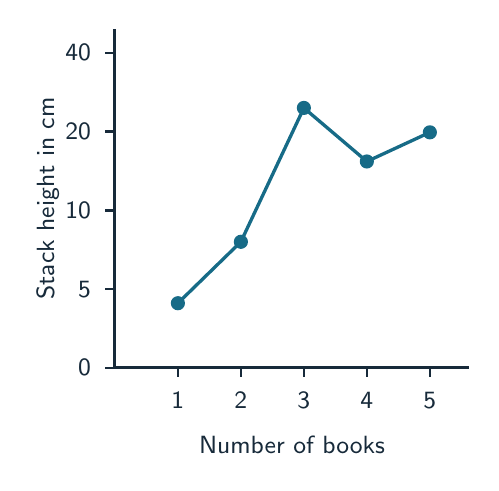
\begin{tikzpicture}[x=1cm,y=1cm]
  \draw[DeckInk, line width=1.1pt] (0,0) -- (4.5,0);
  \draw[DeckInk, line width=1.1pt] (0,0) -- (0,4.3);
  \foreach \x/\v in {0.8/1,1.6/2,2.4/3,3.2/4,4.0/5}{
    \draw[DeckInk, line width=0.9pt] (\x,0) -- (\x,-0.12);
    \node[font=\sffamily\small] at (\x,-0.42) {\v};
  }
  \foreach \y/\v in {0/0,1/5,2/10,3/20,4/40}{
    \draw[DeckInk, line width=0.9pt] (0,\y) -- (-0.12,\y);
    \node[font=\sffamily\small, anchor=east] at (-0.18,\y) {\v};
  }
  \node[font=\sffamily\small] at (2.25,-0.98) {Number of books};
  \node[font=\sffamily\small, rotate=90] at (-0.85,2.15) {Stack height in cm};
  \draw[DeckAccent, line width=1.2pt] (0.8,0.82) -- (1.6,1.60) -- (2.4,3.30) -- (3.2,2.62) -- (4.0,2.99);
  \foreach \p in {(0.8,0.82),(1.6,1.60),(2.4,3.30),(3.2,2.62),(4.0,2.99)}
    \fill[DeckAccent] \p circle (0.09);
\end{tikzpicture}
\end{document}
